\documentclass[journal,12pt,twocolumn]{IEEEtran}
\usepackage{amsthm}
\allowbreak
\usepackage{setspace}
\usepackage{gensymb}
\singlespacing
\usepackage[cmex10]{amsmath}
\usepackage{caption}
\usepackage{amsthm}
\usepackage{float}
\DeclareUnicodeCharacter{2212}{-}
\usepackage{tikz}
\usepackage{pgfplots}

\usepackage{mathrsfs}
\usepackage{txfonts}
\usepackage{stfloats}
\usepackage{bm}
\usepackage{cite}
\usepackage{cases}
\usepackage{subfig}

\usepackage{longtable}
\usepackage{multirow}

\usepackage{enumitem}
\usepackage{mathtools}
\usepackage{steinmetz}
\usepackage{tikz}
\usepackage{circuitikz}
\usepackage{verbatim}
\usepackage{tfrupee}
\usepackage[breaklinks=true]{hyperref}
\usepackage{graphicx}
\usepackage{tkz-euclide}
\graphicspath{ {./images/} }
\usetikzlibrary{calc,math}
\usepackage{listings}
    \usepackage{color}                                            %%
    \usepackage{array}                                            %%
    \usepackage{longtable}                                        %%
    \usepackage{calc}                                             %%
    \usepackage{multirow}                                         %%
    \usepackage{hhline}                                           %%
    \usepackage{ifthen}                                           %%
    \usepackage{lscape}     
\usepackage{multicol}
\usepackage{chngcntr}

\DeclareMathOperator*{\Res}{Res}

\renewcommand\thesection{\arabic{section}}
\renewcommand\thesubsection{\thesection.\arabic{subsection}}
\renewcommand\thesubsubsection{\thesubsection.\arabic{subsubsection}}

\renewcommand\thesectiondis{\arabic{section}}
\renewcommand\thesubsectiondis{\thesectiondis.\arabic{subsection}}
\renewcommand\thesubsubsectiondis{\thesubsectiondis.\arabic{subsubsection}}


\hyphenation{op-tical net-works semi-conduc-tor}
\def\inputGnumericTable{}                                 %%

\lstset{
%language=C,
frame=single, 
breaklines=true,
columns=fullflexible
}
\begin{document}


\newtheorem{theorem}{Theorem}[section]
\newtheorem{problem}{Problem}
\newtheorem{proposition}{Proposition}[section]
\newtheorem{lemma}{Lemma}[section]
\newtheorem{corollary}[theorem]{Corollary}
\newtheorem{example}{Example}[section]
\newtheorem{definition}[problem]{Definition}

\newcommand{\BEQA}{\begin{eqnarray}}
\newcommand{\EEQA}{\end{eqnarray}}
\newcommand{\define}{\stackrel{\triangle}{=}}
\bibliographystyle{IEEEtran}
\raggedbottom
\setlength{\parindent}{0pt}
\providecommand{\mbf}{\mathbf}
\providecommand{\pr}[1]{\ensuremath{\Pr\left(#1\right)}}
\providecommand{\qfunc}[1]{\ensuremath{Q\left(#1\right)}}
\providecommand{\sbrak}[1]{\ensuremath{{}\left[#1\right]}}
\providecommand{\lsbrak}[1]{\ensuremath{{}\left[#1\right.}}
\providecommand{\rsbrak}[1]{\ensuremath{{}\left.#1\right]}}
\providecommand{\brak}[1]{\ensuremath{\left(#1\right)}}
\providecommand{\lbrak}[1]{\ensuremath{\left(#1\right.}}
\providecommand{\rbrak}[1]{\ensuremath{\left.#1\right)}}
\providecommand{\cbrak}[1]{\ensuremath{\left\{#1\right\}}}
\providecommand{\lcbrak}[1]{\ensuremath{\left\{#1\right.}}
\providecommand{\rcbrak}[1]{\ensuremath{\left.#1\right\}}}
\theoremstyle{remark}
\newtheorem{rem}{Remark}
\newcommand{\sgn}{\mathop{\mathrm{sgn}}}
\providecommand{\abs}[1]{$\left\vert#1\right\vert$}
\providecommand{\res}[1]{\Res\displaylimits_{#1}} 
\providecommand{\norm}[1]{$\left\lVert#1\right\rVert$}
%\providecommand{\norm}[1]{\lVert#1\rVert}
\providecommand{\mtx}[1]{\mathbf{#1}}
\providecommand{\mean}[1]{E$\left[ #1 \right]$}
\providecommand{\fourier}{\overset{\mathcal{F}}{ \rightleftharpoons}}
%\providecommand{\hilbert}{\overset{\mathcal{H}}{ \rightleftharpoons}}
\providecommand{\system}{\overset{\mathcal{H}}{ \longleftrightarrow}}
	%\newcommand{\solution}[2]{\textbf{Solution:}{#1}}
\newcommand{\solution}{\noindent \textbf{Solution: }}
\newcommand{\cosec}{\,\text{cosec}\,}
\providecommand{\dec}[2]{\ensuremath{\overset{#1}{\underset{#2}{\gtrless}}}}
\newcommand{\myvec}[1]{\ensuremath{\begin{pmatrix}#1\end{pmatrix}}}
\newcommand{\mydet}[1]{\ensuremath{\begin{vmatrix}#1\end{vmatrix}}}
\numberwithin{equation}{subsection}
\makeatletter
\@addtoreset{figure}{problem}
\makeatother
\let\StandardTheFigure\thefigure
\let\vec\mathbf
\renewcommand{\thefigure}{\theproblem}
\def\putbox#1#2#3{\makebox[0in][l]{\makebox[#1][l]{}\raisebox{\baselineskip}[0in][0in]{\raisebox{#2}[0in][0in]{#3}}}}
     \def\rightbox#1{\makebox[0in][r]{#1}}
     \def\centbox#1{\makebox[0in]{#1}}
     \def\topbox#1{\raisebox{-\baselineskip}[0in][0in]{#1}}
     \def\midbox#1{\raisebox{-0.5\baselineskip}[0in][0in]{#1}}
\vspace{3cm}
\title{AI1103: Assignment 4}
\author{Damaragidda Bharadwaja Rao - CS20BTECH11012}
\maketitle
\newpage
\bigskip
\renewcommand{\thefigure}{\theenumi}
\renewcommand{\thetable}{\theenumi}
Download all python codes from 
\begin{lstlisting}
https://github.com/Bharadwaja-rao-D/AI1103/blob/main/assignment4/assignment4.py
\end{lstlisting}
%
and latex-tikz codes from 
%
\begin{lstlisting}
https://github.com/Bharadwaja-rao-D/AI1103/blob/main/assignment4/assignment4.tex
\end{lstlisting}
\section*{Problem GATE-CS(2015)-Q3(General Aptitude): }
Given set A = \{2,3,4,5\} and set B = \{11,12,13,14,15\}, two numbers are randomly selected , one from each set. What is the probability that sum of two numbers is equal to 16?
\section*{Solution:}
Let X and Y be a random variable which takes values from set A and B respectively.We want to calculate Pr(X+Y=16)
\begin{equation}
  p_X(n)=\begin{cases}
    \dfrac{1}{4}, & \text{if } 2\leq n\leq 5.\\
    0, & \text{otherwise}.
  \end{cases}
\end{equation}
\begin{equation}
  p_Y(n)=\begin{cases}
    \dfrac{1}{5}, & \text{if } 11\leq n\leq 15.\\
    0, & \text{otherwise}.
  \end{cases}
\end{equation}
\begin{align}
&p_z(n) = \Pr(X+Y = n) = \Pr(Y=n-X)\\
&p_z(n) = \sum_k p_x(k)p_y(n-k) = p_x(n) * p_y(n)\\
&p_z(n) = \frac{1}{4} \sum_{k=2}^5 p_y(n-k)=\frac{1}{4}\sum_{k=n-5}^{n-2} p_y(k)
\end{align}
\begin{equation}
  p_z(n)=\begin{cases}
  &0 , n < 13\\
  &\dfrac{1}{20}\times (n-12) ,13 \leq n < 16\vspace{0.2cm}\\
  &\dfrac{1}{20} \times 4 , 16 \leq n \leq 17\vspace{0.2cm}\\
  &\dfrac{21-n}{20} , 18 \leq n \leq 20\vspace{0.2cm}\\
  & 0 ,n > 20
  \end{cases}
\end{equation}
\begin{align}
\therefore p_z(16) = \frac{1}{5}
\end{align}
\begin{figure}[h]
    \centering
    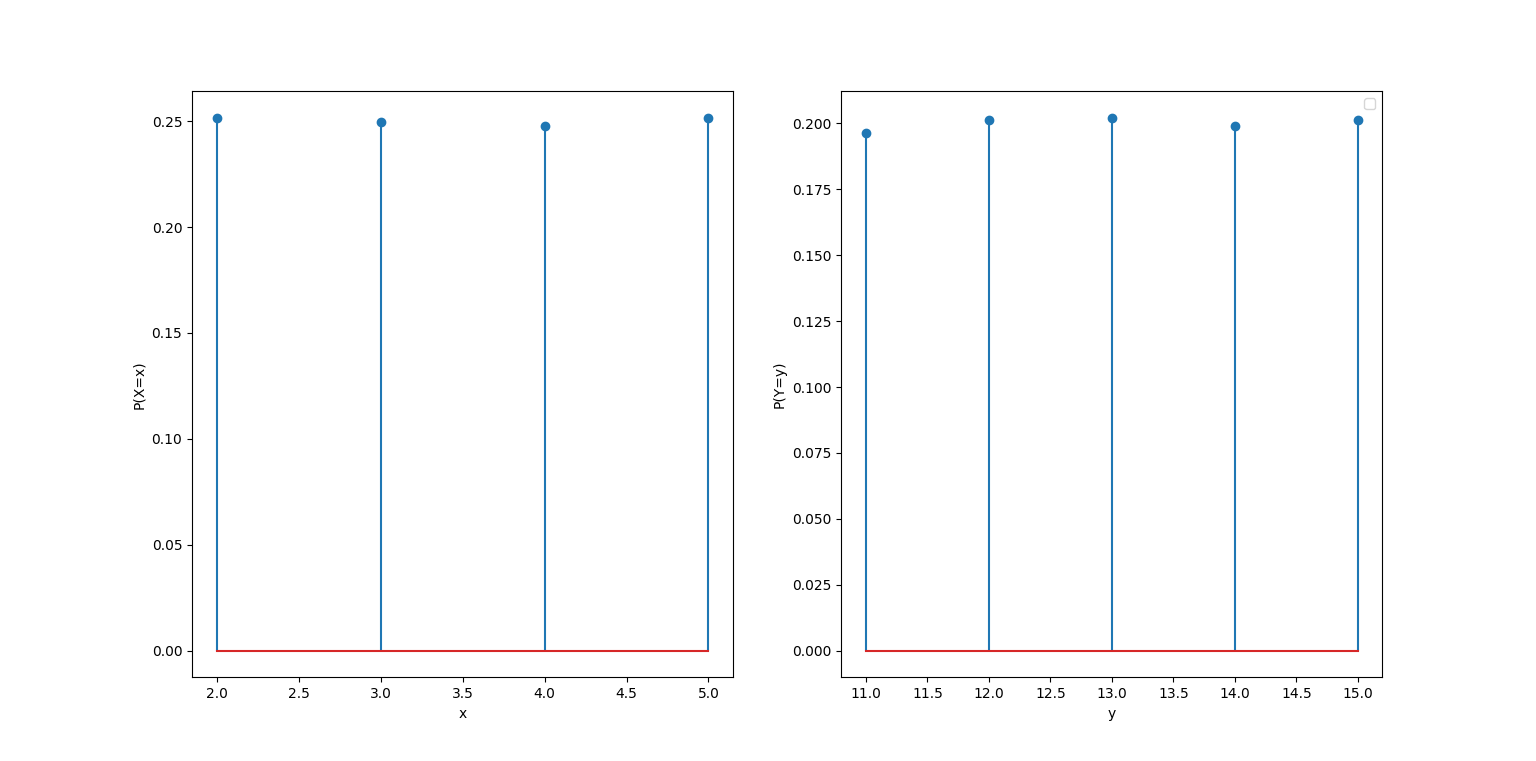
\includegraphics[width=\columnwidth]{assignment4_plot2.png}
\end{figure}
\begin{figure}[h]
    \centering
    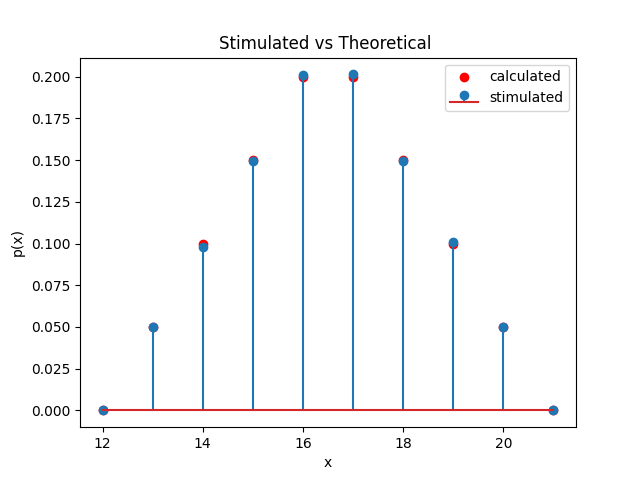
\includegraphics[width=\columnwidth]{assignment4_plot1.png}
\end{figure}
\end{document}
